\documentclass[10pt]{article}
\usepackage[polish]{babel}
\usepackage[utf8]{inputenc}
\usepackage[T1]{fontenc}
\usepackage{graphicx}
\usepackage[export]{adjustbox}
\graphicspath{ {./images/} }

\title{LIGA MATEMATYCZNA im. Zdzisława Matuskiego PAŹDZIERNIK 2018 SZKOŁA PODSTAWOWA }

\author{}
\date{}


\begin{document}
\maketitle
(klasy IV - VI)

\section*{ZADANIE 1.}
W każdym wierzchołku trójkąta umieszczono pewną liczbę, a na każdym boku - sumę liczb z obu jego końców. Znajdź liczby zapisane w wierzchołkach, jeżeli na bokach znajdowały się liczby 1256, 1820, 2018.

\section*{ZADANIE 2.}
Trzej bracia (każdy waży 120 kg ), każdy z żoną (ważącą 60 kg ) i dzieckiem (o wadze 30 kg ) chcą przeprawić się przez rzekę. Na brzegu znaleźli łódkę o ładowności 120 kg . Ile co najmniej razy łódka będzie musiała pokonać drogę od jednego brzegu do drugiego, aby cała rodzina (dziewięć osób) znalazła się na drugim brzegu rzeki? Podczas każdej przeprawy w łódce musi znajdować się przynajmniej jedna osoba dorosła.

\section*{ZADANIE 3.}
Na okręgu umieszczono cztery liczby: 2, 5, 7, 8 (w tej kolejności). Ruch polega na wstawieniu między każdą parę sasiednich liczb ich dodatniej różnicy, a następnie wymazaniu wszystkich starych liczb. Po ilu ruchach po raz pierwszy otrzymamy same zera?

\section*{ZADANIE 4.}
Znajdź wszystkie liczby dwucyfrowe, których iloczyn cyfr jest liczbą pierwszą.

\section*{ZADANIE 5.}
Na poniższym rysunku przedstawiono dziesięciokąt, w którym każde dwa sąsiednie boki są prostopadłe. Długości niektórych boków zostały podane. Oblicz obwód dziesięciokąta.\\
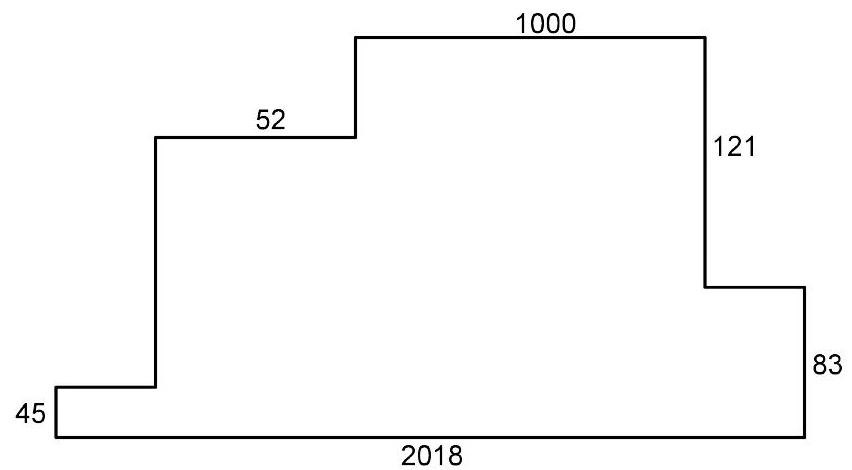
\includegraphics[max width=\textwidth, center]{2024_11_21_7684d66c1edfbb46e8eeg-1}


\end{document}